\documentclass[a4paper,12pt]{article}
\usepackage[utf8]{inputenc}
\usepackage[bitstream-charter]{mathdesign}
\usepackage{ragged2e}
\usepackage[spanish]{babel}%Paquete de caracteres y títulos en español
\usepackage{anysize}%Paquete que permite cambiar márgenes
\marginsize{1cm}{1cm}{2cm}{2cm}
\usepackage{amsmath}%Paquete para insertar símbolos matemáticos
\usepackage{hyperref}%Paquete para insertar referencias en el texto
\usepackage{textcomp,gensymb}
\usepackage{float}%Paquete para tratar figuras y tablas como flotantes
\usepackage{lipsum}%Paquete para insertar texto mudo
\usepackage{graphicx}
\usepackage{caption}
\usepackage{subcaption}
\usepackage{url}%Paquete para insertar URL's
\usepackage{multicol}%Paquete para crear ambientes multicolumna
\setlength\columnsep{18pt}%Especifíca separación de las columnas
\renewenvironment{abstract}%Modifica el ambientes abstract para modificar la alineación
 {\par\noindent\textbf{\abstractname}\ \ignorespaces \\}
 {\par\noindent\medskip}

\title{INFORME X}
%-----------------------------------------------------------------------------------------------------------------------------------------

\begin{document}

\begin{center}
\Large\underline{RFID Middleware Design and Architecture}
\vspace{0.4cm}

\normalsize
Surya.S
\vspace{0.1cm}

\textit{\small{Artificial Intelligence and Data Science }\\
\small{Shiv Nadar University Chennai}}
\vspace{0.1cm}
\small{Email :- surya21110199@snuchennai.edu.in}
\medskip

\normalsize

\end{center}
%-----------------------------------------------------------------------------------------------------------------------------------------

\medskip

%-----------------------------------------------------------------------------------------------------------------------------------------
\begin{multicols}{2}
%------------------------------------------------------------------------
\section{Abstract}
RFID middleware is a software layer that acts as an intermediary between RFID readers and back-end systems, enabling the seamless integration of RFID technology into various applications. This paper presents a comprehensive research on the design and implementation of RFID middleware, including its architecture, key components, and functionality. The study also examines the challenges and limitations of RFID middleware, as well as potential solutions to overcome these issues. Additionally, the paper explores various use cases of RFID middleware in different industries, such as supply chain management, retail, and healthcare, and discusses the benefits and potential impact of RFID middleware on these industries. The research concludes with recommendations for future work in the field of RFID middleware design and development..\\
\\
\textbf{keywords:}
RFID middleware, design, implementation, architecture, key components, functionality, challenges, limitations, solutions, use cases, supply chain management recommendations, future work..
%--------------------------------------------------------------------------------
\section{Introduction}
Radio Frequency Identification (RFID) is a form of Automatic Identification and Data Capture (AIDC) technique (Ishikawa et al., 2003). RFID is recently being used in a wide range of areas such as Supply Chain Management (SCM), health care, traffic monitoring, retail, and access control (Polniak, 2007). The ability to store large amounts of data and identify items which are not in the line of sight has given RFID technology an edge over other automatic identification approaches such as the barcode based systems (Ishikawa et al., 2003) and optical character recognition systems (OCR) (Phoenix Software International, 2006). As an example, RFID technology integration in SCM systems has resulted in the reduced losses and improved visibility in various stages of supply chaining (Sheng et al., 2008), reduced numbers of data entry errors, efficient inventory management, and lower human labor costs in distribution centers (Tutorial-Reports, 2007).

A binary code comprising a field of bars and gaps arranged in parallel configuration is used by the barcode based identification systems. The analysis of the reflected beam on the bar gaps, allows the numerical and alphanumerical interpretation of the barcode sequence made up of narrow and wide bars. The interpreted value obtained specifies a unique code that is used for object identification. The disadvantage of the barcode system is that the barcode needs to be aligned in order to be read by the laser scanner (Ishikawa et al., 2003). The OCR based systems consist of optical machine readers used to recognize alphanumeric codes which are placed on the objects to be uniquely identified. The drawbacks of this system consist of the cost of operation, and the complexity of the OCR readers (Phoenix Software International, 2006).

The RFID systems basically consist of three elements: a tag/transponder, a reader and a middleware deployed at a host computer. The RFID tag is a data carrier part of the RFID system which is placed on the objects to be uniquely identified. The RFID reader is a device that transmits and receives data through radio waves using the connected antennas. Its functions include powering the tag, and reading/writing data to the tag. As shown Fig. 1, the signals sent by the reader‘s antennas form an interrogation zone made up of an electromagnetic field. When a tag enters this zone, it gets activated to exchange data with the reader (Al-Mousawi, 2004). Later, the identification data read by the RFID reader is processed by the software system, known as the RFID middleware. The RFID middleware manages readers, as well as filters and formats the RFID raw tag data so that they can be accessed by the various interested enterprise applications (Floerkemeier& Lampe, 2005). Hence, the middleware is a key component for managing the flow of information between tag readers and enterprise applications (Burnell, 2008)..\\

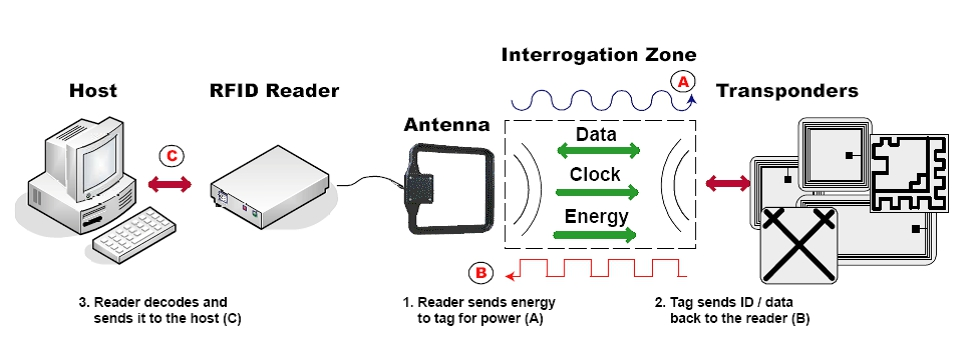
\includegraphics[width=8cm,height=10cm,keepaspectratio]{Surya-RFID/image1.jpg}

\section{ RFID system components}
RFID systems are produced by many manufacturers and exist in countless variants. However, a RFID system consists mainly of three components; the transponder/tag, reader, and RFID middleware.
\\
\item \textbf {1)	RFID transponder}\\
\\
A RFID transponder, or tag, consists of a chip and an antenna. A chip can store a unique serial number or other information based on the tag‘s type of memory. The tag‘s type of memory can be read-only, read-write, or write-once and read-many (United States Government Accountability Office, 2005). Read-only tags are much cheaper to produce and are used in most current applications. Read-write tags are useful when information needs to be updated (Al-Mousawi, 2004). The antenna is used to transmit information from the chip to the reader, and the larger the antenna the longer the read range. The RFID tag can be either attached or embedded in an object to be identified, and can be scanned by mobile or stationary readers using radio waves (United States Government Accountability Office, 2005).


\\
\item \textbf {2)	Passive tags}\\
\\
Present the simplest version of RFID tags which do not contain their own power source, such as a battery, and cannot initiate communication with the reader. The passive tag derives its power from the energy waves transmitted by the reader and responds to the reader‘s radio frequency emissions, therefore the passive tag relies entirely on the reader as its power source. A passive tag should store, at a minimum, a unique identifier for the item tagged, and can be read from a range of about 10 to 20 feet under perfect conditions (United States Government Accountability Office, 2005). Passive tags have lower production costs, meaning that they can be applied to less expensive disposable goods (e.g. a bottle of shampoo).

The cost of passive tags varies based on the radio frequency used, amount of memory, and design of the antenna, and other tag requirements. Passive tags can operate at low, high, ultrahigh, or microwave frequency. The development of passive RFID tags has made wide scale use of them in many organizations. Examples of passive tag applications include mass transit passes, building access badges, and consumer products in the supply chain (United States Government Accountability Office, 2005).


\\
\item \textbf  {3)	Active tags}\\
\\
Unlike passive tags, active tags contain a power source and a transmitter, in addition to the antenna and chip, and send a continuous signal. These tags typically have read/write capabilities; tag data can be rewritten and/or modified. Active tags can initiate communication and communicate over longer distances up to 750 feet, depending on the battery power. Because these tags contain more hardware than passive RFID tags, they are more expensive and are reserved for costly items that are read over greater distances (United States Government Accountability Office, 2005). RFID manufacturers typically do not quote prices for active tags without first determining their storage type and quantity, and range.


\\
\item \textbf{4)	Semi passive tags}\\
\\
This type of tags is called also semi-active tags. Semi-passive tags do not initiate communication with the reader but contain batteries that allow the tag to perform other functions, such as monitoring environmental conditions and powering the tag‘s internal electronics. In order to conserve battery life, some semi-passive tags do not actively transmit a signal to the reader. Instead, they remain dormant until they receive a signal from the reader. Semi-passive tags can be connected to sensors to store information for container security devices (United States Government Accountability Office, 2005). Semi-passive tags have the middle transmission range and cost (Vacca, 2009).

As a summary, passive tags are consequently much lighter than active tags, less expensive, and offer a virtually unlimited operational lifetime. The trade off is that they have shorter read ranges than active tags and require a higher-powered reader (Association for Automatic Identification and Mobility, n.d.). Table 1 shows a comparison among passive, semi-passive, and active tags.

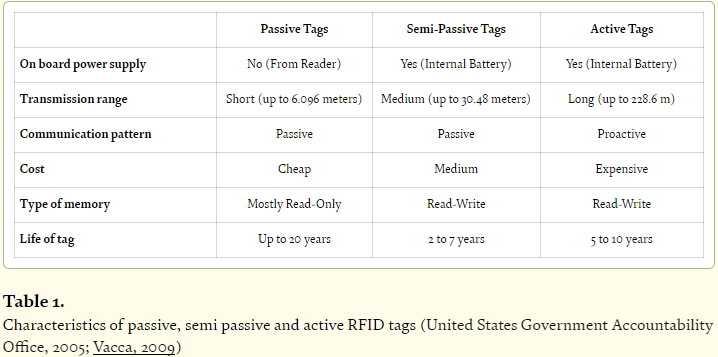
\includegraphics[width=9cm,height=12cm,keepaspectratio]{Surya-RFID/table1.png}

\section{RFID middleware}
\\
The middleware refers broadly to software or devices that connect RFID readers and the data they collect, to enterprise information systems. RFID middleware helps making sense of RFID tag reads, applies filtering, formatting and logic to tag data captured by a reader, and provides this processed data to back-end applications (Burnell, 2008). RFID middleware serves in managing the flow of data between tag readers and enterprise applications, and is responsible for the quality, and therefore usability of the information. It provides readers connectivity, context-based filtering and routing, and enterprise / B2B integration. RFID middleware design and components will be discussed further in the next sections.

When designing a RFID middleware solution, the following issues need to be considered:

Multiple hardware support: The middleware must provide a common interface to access different kinds of hardware offering different features. Synchronization and scheduling: There should be intelligent scheduling and synchronization among all the processes of the middleware. This minimizes the latency and improves the efficiency of the middleware. Real-time handling of incoming data from the RFID readers: The middleware should handle the huge amount of data captured by the connected readers in real time without read misses. Interfacing with multiple applications: The middleware should be capable of interacting with multiple applications simultaneously, by catering to all the requirements of the applications with minimal latency.Device neutral interface to the applications: The application developer should only use the generic set of interfaces provided by the middleware independently of the type of hardware connected to the system. Scalability: The middleware design must allow easy integration of new hardware and data processing features.

\section{RFID middleware components}
\\
A RFID middleware is the interface that sits between the RFID hardware and RFID applications. It provides the following advantages:
\begin{itemize}
\item[$\blacksquare$] It hides the RFID hardware details from the applications.
\item[$\blacksquare$] It handles and processes the raw RFID data before passing it as aggregated events to the applications.
\item[$\blacksquare$] It provides an application level interface for managing RFID readers and querying the RFID data.
\end{itemize}

\vspace{10pt}


A layer of the RFID middleware incorporates all the device drivers of different hardware and exposes to the application standard interfaces to access this hardware. If the application was provided with all the device drivers of all connected readers, it will be a hard job to manage and interface each of the devices. The application developer will then need to understand all the hardware specific internals and operations. Also, the application, if provided with the huge amount of raw tag data reported by the readers, will find it very difficult to process the data in real time. A RFID middleware provides a standardized way of dealing with this flood of information, which processes the raw data and provides the application with clean and filtered data.
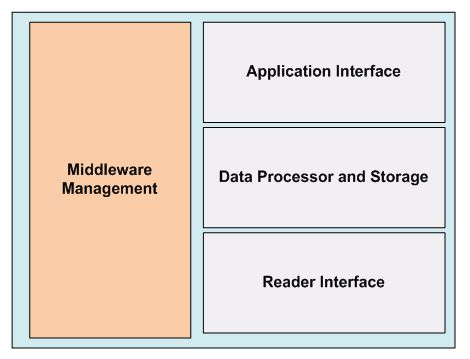
\includegraphics[width=8cm,height=10cm,keepaspectratio]{Surya-RFID/image2.jpg}


\\
\item \textbf{1) Reader Interface	}\\
\\
The reader interface is the lowest layer of the RFID middleware which handles the interaction with the RFID hardware. It maintains the device drivers of all the devices supported by the system, and manages all the hardware related parameters like reader protocol, air interface, and host-side communication.

\\
\item \textbf{2) Data processor and storage	}\\
\\
The data processor and storage layer is responsible for processing and storing the raw data coming from the readers. Examples of processing logic carried by this layer are data filtering, aggregation, and transformation. This layer also processes the data level events associated with a specific application.

\\

\item \textbf{3) Application interface	}\\
\\
The application interface provides the application with an API to access, communicate, and configure the RFID middleware. It integrates the enterprise applications with the RFID middleware by translating the applications’ requests to low level middleware commands.

\\

\vfill
\item\textbf{Excisting RFID Middleware}\\


\\
In this section, we present the main RFID middleware
systems and review their key features and capabilities
\pagebreak



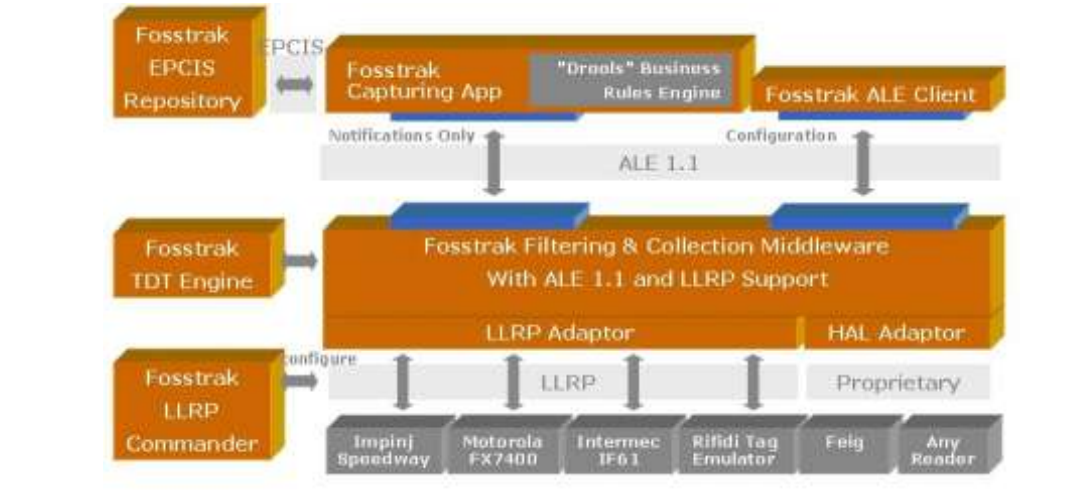
\includegraphics[width=17cm,height=9cm]{Surya-RFID/exmid2.png}

\\

\item \textbf{1) Aspire Middleware	}\\
\\
The structure of the Advanced Sensors and lightweight
Programmable middleware for Innovative RFID Enterprise
applications (Aspire) middleware is shown in Figure 3 .
Aspire consists of various layers as follows. The Hardware
abstraction layer (HAL) unifying the way of interaction with
multiple readers dealing and interacting with multiple
protocols. Its implementation is divided into different
modules (for reader simulators and one for each reader
manufacturer). The Reader Core Proxy (RCP) layer is
located between the readers and the ALE, and it helps in the
communication between reader supporting protocol X and
corresponding Filtering and Collection reader protocol
interface (RP, LLRP). ALE layer converts data from its raw
form to reports by collecting relevant information and
creating reports that are being subscribed at by applications,
Business Event Generator (BEG), between the Filtering and
Collection and Information Sharing. ALE layer can be seen
as a specific instance of an EPC-IS capturing application that
parses EPC-ALE reports. It fuses these reports with business
context data using the assigned business event from the
company’s business metadata to serve as guide and
accordingly prepares EPC-IS compliant events.
\\

\\
\vspace{89mm} %5mm vertical space

\item \textbf{2) FOSSTrak Middleware	}\\
\\
The structure of the Free and Open-Source Software for
Track and Trace (FOSSTrack) is shown in Figure 4 .
FOSSTrack consists of four separate modules: (i) EPCIS
Repository that enables users to exchange EPC-related data
with trading partners through the EPCglobal Network, (ii)
Tag Data Translation (TDT) Library that translates one
representation of EPC into another representation, (iii)
Filtering and Collection Middleware with ALE and LLRP
Support. It takes the EPC network role of data filtering and
aggregation. It also provides report generation and generating
events for the EPCIS repository, and (iv) LLRP Commander
that describes an interface between RFID readers and clients
that provide means to command an RFID Reader to inventory
tags (read the EPC codes carried on tags), read tags (read
other data on the tags a part from the EPCcode), write tags,
and execute other protocol-dependent access commands
(such as ‘kill’ and ‘lock’ from EPCglobal Class 1 Generation
2). However, the standard defines how to retrieve reader device capabilities and facilitate the addition of support for
new air protocols.
\\

\item\textbf{3) ACCADA Middleware}\\
\\
ACCADA  consists of three separate modules. The
Reader module implements the EPCglobal Reader Protocol,
which includes collecting, filtering, time aggregates and
space aggregates and also supports write on tags. The Accada
reader implementation can be used in three different modes
the reader implementation which is deployed on a separate
server using the built-in HAL in simulation mode to facilitate
testing of RFID applications and scheduling detection. It can
also be deployed on an RFID reader itself to provide data
dissemination, filtering, and aggregation capabilities.
The Filtering and Collection Middleware module allows
applications to define a subscription and create a report that is
sent according to a pre-determined schedule to the subscribed
applications. The interface between the filtering and
collection middleware and a host application is based on the
EPCglobal ALE Specification.
\\
\\
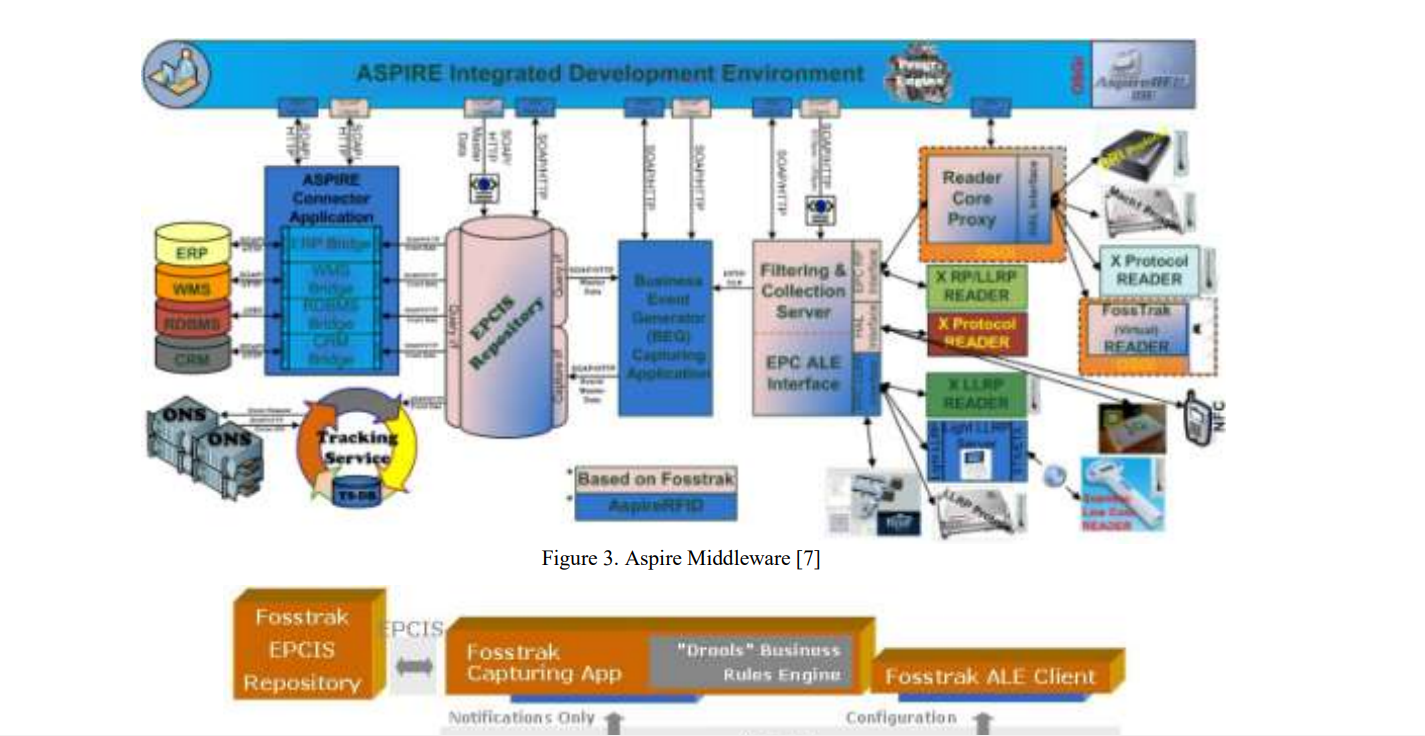
\includegraphics[width=8cm,height=10cm,keepaspectratio]{Surya-RFID/exmid.png}

\item\textbf{4)CUHK Middleware}\\
\\
CUHK  is a flexible and cost-effective solution for
RFID network deployment and configuration which follows
EPCglobal and the ALE specifications. CUHK is designed as
J2EE application hosted in JBoss server and connected
database with JDBC. Users can access the RFID network
using ALE Interface extended to support two functions read
and write into the tag memory. Through Management console
user can configure, control, manage and monitor all readers
in RFID network. CUHK provides five basic functions: (i)
Data Acquisition, allows receiving EPCs from one data
source to another, (ii) Collecting data in time intervals, (iii)
Filtering, that eliminates duplicate data and filters the needed
EPCs, (iv) Manipulating data to reduce the volume of data,
and (v) Report Generation using ALE API which allows
users to specify in a high level what data is needed and in
which format, and generate ECReports for given Event cycle

\item\textbf{4)LIT Middleware}\\
\\
Logistics Information Technology (LIT)  implements
the concepts of both ALE and EPCIS layers of the EPCGlobal standard. The ALE layer consists of four sub layers:
\begin{itemize}
\item  Application Abstraction Layer (AAL),
\item  State-based Execution Layer.
\item  Continuous Query Layer, and
\item  Reader Abstraction Layer.
\end{itemize}

These sub-layers perform the base role of the ALE layer of
grouping, filtering data, duplicate removal and hardware
abstraction. The EPCIS layer, which represents the business
layer and is the connection to applications.

\item\textbf{5) WinRFID}
\\
The main components of the WinRFID founded by
UCLA (RFID research at WINMEC: Wireless Internet for
Mobile Enterprise Consortium) are shown in Figure 5 [15]. It
is developed on Microsoft .NET framework composed of
five main layers each of different responsibilities
i)Physical layer that deals with the hardware/readers, tags and
other sensors, 
(ii) Protocol Layer that abstracts the reader-tag
protocols, 
(iii) Data processing layer that process the data
streams generated by the reader network and filtering them,
(iv) XML Framework that handles data and information
representation, and 
(v) Data presentation that presents data
based on the requirements of the end-users or different
enterprise applications.

\pagebreak

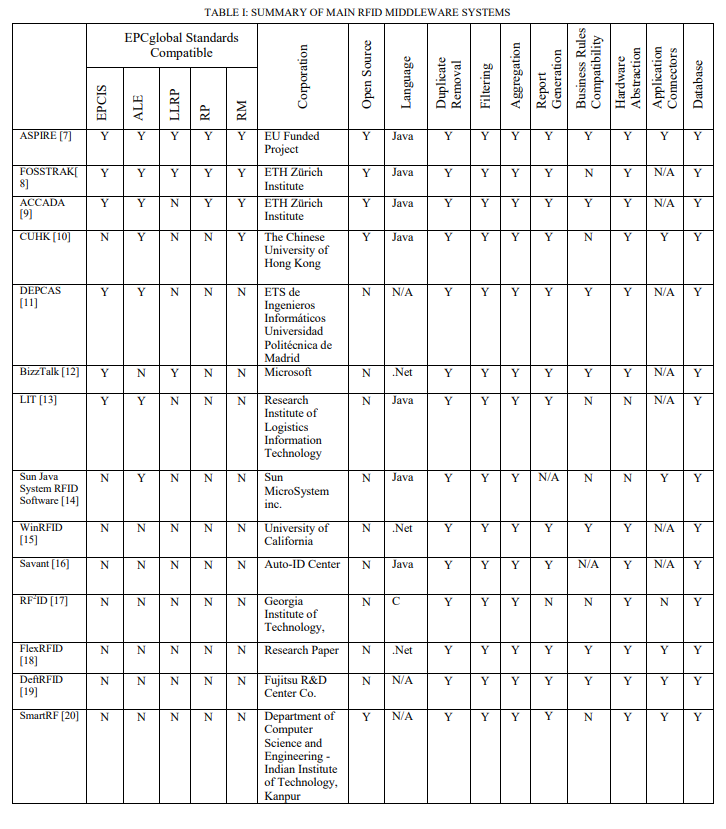
\includegraphics[width=20cm,height=20cm,keepaspectratio]{Surya-RFID/tablee.png}

\pagebreak







\section{Conclusion}
A number of enterprise applications using RFID technique introduce a need for an infrastructure that hides proprietary device interfaces, facilitates configuration and monitoring of the devices, and processes the captured data. This chapter introduces RFID middleware and its design issues, presents some existing middleware solutions, and details the FlexRFID middleware framework that we developed to address the application requirements stated above. FlexRFID has four important layers: the Device Abstraction Layer (DAL), the Business Event and Data Processing Layer (BEDPL), and the Application Abstraction Layer (AAL). FlexRFID enables the following: communication with different types of devices; implementation of functionalities by ensuring the business rules using policy-based management; and seamless integration of various enterprise applications. The smart library application has been developed to show the usefulness of the designed middleware solution. Also the scenarios of integrating FlexRFID with an inventory management application have been set.

With respect to the future work we intend to develop all the possible scenarios and specific events that could be triggered in an SCM application for inventory control, integrate the FlexRFID middleware with an open source system for inventory control (e.g. TechLogic Inventory Control System, Opentaps…), and show how the different layers of FlexRFID middleware will work to deliver enhanced visibility of inventory in various stages of supply chaining.

Next we are intending to integrate FlexRFID with a healthcare application, and in the context of Situational Awareness; being aware of what is happening around users and understand how information, events, and actions will impact their goals, both now and in the near future. This will allow us to evaluate the FlexRFID middleware with multiple hardware configurations and applications’ requirements.


%--------------------------------------------------------------------------------------------------
\end{multicols}
%----------------------------------------------------------------------------------


\end{document}